\documentclass[14pt]{extarticle}
\usepackage{fontspec}
\usepackage{polyglossia} % use instead of babel
\usepackage{pgfplots}
\setdefaultlanguage{hebrew}
\setotherlanguage{english}
\newfontfamily\hebrewfont[Script=Hebrew]{Arial}

% TODO: figure out if better to keep this or not, for word document pdf output similarity
\usepackage[margin=1in]{geometry}

% might be useful to ensure similarity to word document pdf output
% \usepackage{setspace}
% \singlespacing

% Reset equation counter at the start of each section
\usepackage{chngcntr}
\usepackage{etoolbox}
\counterwithin*{equation}{section}
\preto{\section}{\setcounter{equation}{0}}


\begin{document}

\begin{center}
    {\LARGE \textbf{ממ"ן 12}}\\
    {\textbf{אופטיקה גיאומטרית}}
\end{center}

\begin{itemize}
    \item מגישים: תומר רוזנלפלד, שי רואימי
    \item תאריך ביצוע הניסוי: 19 יולי 2025
    \item מדריך הניסוי: ד"ר סילביו ריינהורן
\end{itemize}

\section*{מטרות הניסוי:}
\begin{enumerate}
    \item מדידת מקדם השבירה בפרספקס
    \item מדידת מרחק מוקד בעדשה מרכזת ועדשה מפזרת
\end{enumerate}

\section*{ניסוי 1 - חוק סנל}
\subsection*{מטרת הניסוי}
מציאת מקדם השבירה של פקספקס 

\subsection*{רקע תיאורטי}
במעבר אור מתווך חומר אחד לאחר, זווית השבירה תלויה במקדם השבירה של שני החומרים, ובזווית הפגיעה.
חוק סנל מתאר את הקשר בין זוויות השבירה והכניסה של האור בחומרים שונים.
מקדם שבירה מוגדר בנוסחא:

\begin{equation}
    n = \frac{c}{v}
\end{equation}

כאשר $c$ היא מהירות האור בריק ו-$v$ היא מהירות האור בחומר.


חוק סנל קובע את הקשר בין זוויות השבירה והכניסה של האור בחומרים שונים:

\begin{equation}
n_1 \sin(\theta_1) = n_2 \sin(\theta_2)
\end{equation}

כאשר $n_1$ ו-$n_2$ הם מקדמי השבירה של החומרים 1 ו-2, ו-$\theta_1$ ו-$\theta_2$ הן זוויות הפגיעה והשבירה בהתאמה.

\subsection*{מערכת המדידה ומהלך הניסוי}

כיוונו קרן אור כלפי חצי דסקה עשויה פרספקס, ובעזרת מד זווית מדדנו את זוויות השבירה בהנתן זוויות פגיעה שונות. בעזרת תוצאות המדידה מצאנו את מקדם השבירה של הפרספקס.

הניסוי נעשה בעזרת מנסרה חצי עגולה. צורה זו משרתת את הניסוי בכך שכאשר קרן האור יוצאת מהמנסרה אינה "נשברת", כי זווית הפגיעה תמיד 0 מעלות, כי רדיוס במעגל ניצב תמיד למשיק למעגל בנקודת ההשקה.

\subsection*{תוצאות וניתוח}

מדידת זווית השבירה בהינתן זווית פגיעה שונה, הובילה לתוצאות הבאות:
\begin{center}
    {\small
    \begin{tabular}{|c|c|c|c|}
    \hline
    זווית פגיעה (מעלות) & זווית שבירה (מעלות) & סינוס זווית פגיעה & סינוס זווית שבירה \\ \hline
    10 & 7   & 0.1736 & 0.1219 \\ \hline
    20 & 13.5 & 0.3420 & 0.2334 \\ \hline
    30 & 20  & 0.5000 & 0.3420 \\ \hline
    40 & 26  & 0.6428 & 0.4384 \\ \hline
    50 & 31  & 0.7660 & 0.5150 \\ \hline
    60 & 36  & 0.8660 & 0.5878 \\ \hline
    70 & 40  & 0.9397 & 0.6428 \\ \hline
    80 & 43  & 0.9848 & 0.6820 \\ \hline
    \end{tabular}
    }
\end{center}

\begin{figure}[ht]
  \centering
  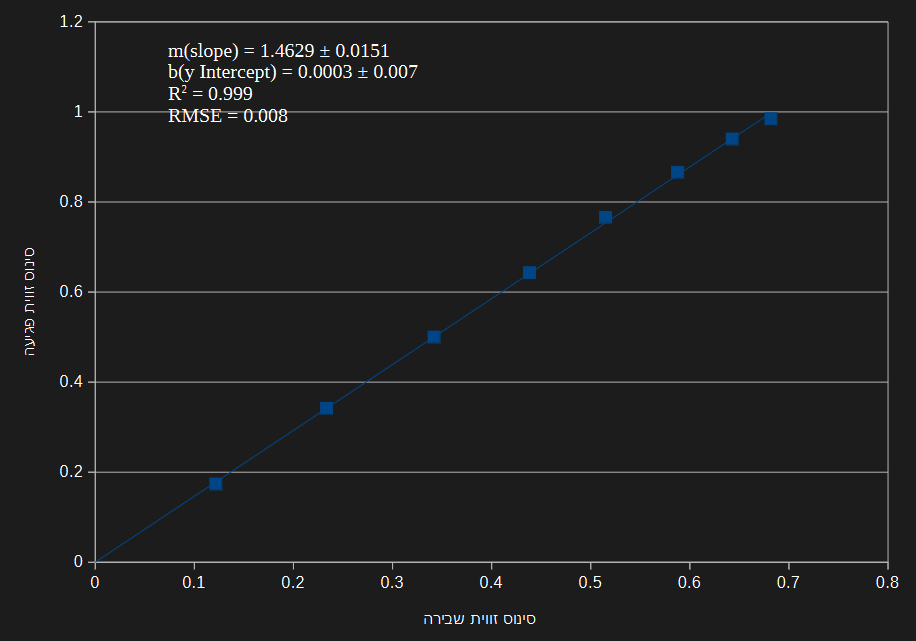
\includegraphics[width=0.8\textwidth]{Lab_1_Experiment_1.png}
  \caption{גרף המתאר את סינוס זווית הפגיעה כתלות בסינוס זווית השבירה}
  \label{fig:excel_chart}
\end{figure}

\subsection*{תוצאות הניסוי וניתוח התוצאות}
על מנת למצוא את מקדם השבירה נעזר בנוסחא:
\begin{equation}
n_{perspex} = \frac{n_{air} * \sin(\theta_1)}{\sin(\theta_2)}
\end{equation}
כאשר $n_{air}$ הוא מקדם השבירה של האוויר ($n_{air}=1$), $\theta_1$ היא זווית הפגיעה ו-$\theta_2$ היא זווית השבירה. נקבל:
\begin{equation}
n_{perspex} = \frac{\sin(\theta_1)}{\sin(\theta_2)}
\end{equation}

נצייר את הנקודות שהתקבלו במדידות בגרף, קיבלנו גרף ליניארי כאשר שיפוע הגרף הוא מקדם השבירה של הפרספקס. קיבלנו את הערך 1.46.

\subsection*{דיון ומסקנות}
הניסוי הצליח להדגים את חוק סנל ואת הקשר בין זוויות השבירה והכניסה של האור בחומרים שונים.

הערך הידוע בספרות הוא  1.49 (אתר אינטרנט - ,(https://refractiveindex.info השגיאה היחסית היא 2.02\%, וככל הנראה נובעת מ:
\begin{itemize}
    \item שגיאת המדידה של מד הזווית היא 0.5 מעלות
    \item רוחב קרן האור
    \item דיוק בתהליך המדידה
\end{itemize}

\section*{ניסוי 2 - החזרה גמורה}
\subsection*{מטרת הניסוי}
מציאת מקדם השבירה של פרספקס באמצעות מציאת הזווית הקריטית

\subsection*{רקע תיאורטי}
כאשר קרן אור פוגעת בחומר בעל מקדם שבירה גבוה יותר, היא נשברת בזווית מסוימת. כאשר זווית זו עולה על זווית מסוימת, הקרן אינה נשברת אלא מוחזרת לחלוטין. זווית זו נקראת הזווית הקריטית.

\subsection*{מערכת המדידה ומהלך הניסוי}

הפעם נהפוך את חצי המנסרה, כאשר קרן האור עוברת מאוויר לפרספקס לא תהיה שבירה (זווית פגיעה 0), והשבירה תקרה כאשר הקרן עוברת מפרספקס לאוויר.

נסובב את המנסרה עד מציאת הזווית הקריטית, ובעזרתה נמצא שוב את מקדם השבירה של הפרספקס.

\subsection*{תוצאות וניתוח}
מצאנו כי זווית השבירה הקריטית היא 42 מעלות. בעזרת נוסחאת סנל, נוכל למצוא את מקדם השבירה של הפרספקס:
\begin{equation}
n_{perspex} = \frac{n_{air}}{\sin(42)}
\end{equation}
כאשר $n_{air}$ הוא מקדם השבירה של האוויר ($n_{air}=1$) ו-42 היא הזווית הקריטית. נקבל:
\begin{equation}
n_{perspex} = \frac{1}{\sin(42)} \approx 1.49
\end{equation}

\subsection*{דיון ומסקנות}
בעזרת מציאת הזווית הקריטית הצלחנו למצוא את מקדם השבירה של הפרספקס, והגענו לערך קרוב יותר לערך הידוע בספרות, שהוא 1.49.

\section*{ניסוי 3 - עדשות}
\subsection*{מטרת הניסוי}
מציאת מרחק המוקד של עדשה מרכזת
\subsection*{רקע תיאורטי}
עדשות הן אובייקטים אופטיים המיועדים לשנות את כיוון קרני האור העוברים דרכם.
מרחק המוקד של עדשה הוא המרחק בין העדשה לנקודה בה מתרכזות קרני האור העוברים דרכה.

נוסחאת גאוס היא נוסחא המתארת את הקשר בין מרחק המוקד של העדשה, המרחק בין העדשה לאובייקט והמרחק בין העדשה לתמונה המתקבלת:
\begin{equation}
\frac{1}{f} = \frac{1}{u} + \frac{1}{v}
\end{equation}
כאשר $f$ הוא מרחק המוקד, $u$ הוא המרחק בין העדשה לאובייקט ו-$v$ הוא המרחק בין העדשה לתמונה המתקבלת.


\end{document}